\documentclass{beamer}
\usepackage[french]{babel}
\usepackage{hyperref}
\usepackage[T1]{fontenc}

\mode<presentation>
{
  \usetheme{Frankfurt}
  \setbeamercovered{transparent}
  \set
}

\setbeamertemplate{footline}{%
  \hfill%
  \usebeamercolor[fg]{page number in head/foot}%
  \usebeamerfont{page number in head/foot}%
  \insertframenumber / \inserttotalframenumber%
  \hspace*{0.5cm}% Adjust this space as needed
  \vskip2pt%
}

%package for plots
\usepackage{booktabs}

\usepackage{tikz}
\usetikzlibrary{shapes.geometric, arrows}
\tikzstyle{startstop} = [rectangle, rounded corners, minimum width=3cm, minimum height=1cm, text centered, text width = 10cm, draw=black, fill=white]
\tikzstyle{process} = [rectangle, minimum width=3cm, minimum height=1cm, text centered, text width = 6cm, draw=black, fill=white, text width = 10cm]
\tikzstyle{arrow} = [ultra thick,->,>=stealth]

\usepackage{xcolor}
\usepackage[skip=2pt,font=normalsize]{subcaption}
\usepackage{adjustbox}

% other packages
\usepackage{latexsym,amsmath,xcolor,multicol,booktabs,calligra}
\usepackage{graphicx,pstricks,listings,stackengine}
\usepackage{wrapfig}


\author{Léo Tarbouriech and Joseph Touzet}
\title{Restricted Boltzman Machines}
\institute{Machnie Learning \\ M2 PCS}
\date{\today}
%\usepackage{GUET}
% \logo{\includegraphics[width=0.5 cm]{Guet-logo.pdf}} % 每一页添加logo

% defs
\def\cmd#1{\texttt{\color{red}\footnotesize $\backslash$#1}}
\def\env#1{\texttt{\color{blue}\footnotesize #1}}
\definecolor{deepblue}{rgb}{0,0,0.5}
\definecolor{deepred}{rgb}{0.6,0,0}
\definecolor{deepgreen}{rgb}{0,0.5,0}
\definecolor{halfgray}{gray}{0.55}

\lstset{
    basicstyle=\ttfamily\small,
    keywordstyle=\bfseries\color{deepblue},
    emphstyle=\ttfamily\color{deepred},    % Custom highlighting style
    stringstyle=\color{deepgreen},
    numbers=left,
    numberstyle=\small\color{halfgray},
    rulesepcolor=\color{red!20!green!20!blue!20},
    frame=shadowbox,
}

\graphicspath{{./Figures/}} 

% ------------------------------------------------------------------------------------------
%     Document
% ------------------------------------------------------------------------------------------
\begin{document}





\begin{frame}
    \titlepage
\end{frame}





\begin{frame}
    \tableofcontents[sectionstyle=show,subsectionstyle=show,subsubsectionstyle=show/shaded/hide]
\end{frame}

\section{RBM and EBM}
\subsection{Energy Based Models (EBM)}
\begin{frame}{Energy Based Models (EBM)}
\begin{itemize}
\item[•] Learn correlations between features
\item[•] Assume we do not know anything about the correlations
\item[•] Two point correlations are sufficients because the model is fully connected
\item[•] Recall statistical field theory course --> fully connected lattice $\leftrightarrow$ only gaussian terms matters
\end{itemize}
\begin{eqnarray*}
	H & = & - \sum_{i = 1}^{N_{features}} - \frac{1}{2} \sum_{i,j} v_i J_{ij} v_j \\
	p(\mathbf{v} \vert \left\{a_i, J_{ij}\right\}) & = & \frac{1}{Z} \exp\left( \sum_{i} a_i v_i + \sum_{ij} v_i J_{ij} v_j \right)
\end{eqnarray*}


\begin{itemize}
\item[•] $J_{ij}$ is a fully connected random matrice
\end{itemize}
\end{frame}





\subsection{Hopfield model and Restricted Boltzman Machines}
\begin{frame}{RBM and EBM}{Hopfield model and Restricted Boltzman Machines}

\begin{itemize}
\item[•] In an Hopfield model we would have $J_{ij} = W_{i\mu} W_{j\mu}$
\item[•] With $W_{i\mu}= \{ -1,+1 \}$
\item[•] This model is know to be able to "remember patterns"
\item[•] Hard to train, does not converge appart for very simple situations --> Few patterns
\item[•] Slow to sample if the system is very big.
\end{itemize}
\center{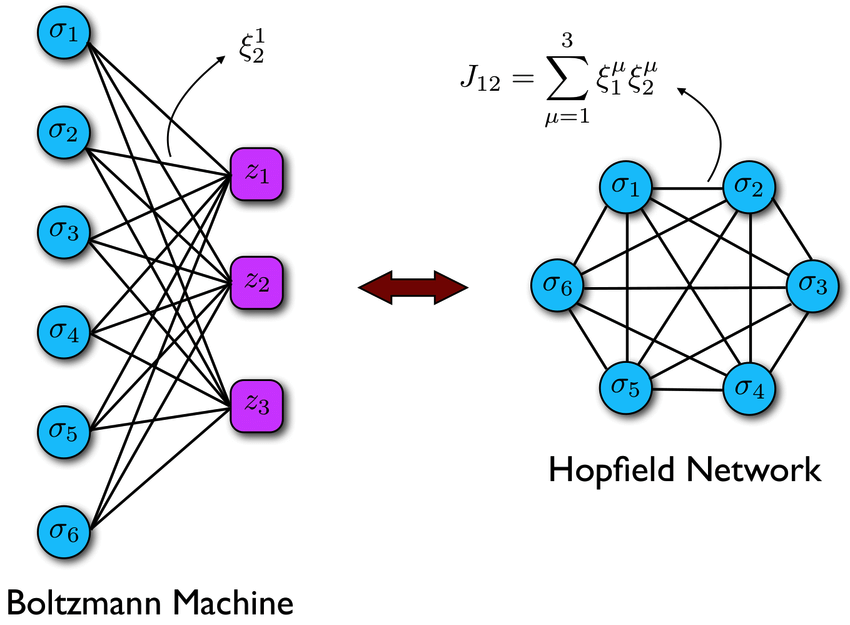
\includegraphics[width=0.5\textwidth]{Slides/Restricted-Boltzmann-machine-and-associative-Hopfield-network-Left-panel-example-of-a.png}}
\end{frame}


\begin{frame}{RBM and EBM}{Hopfield model and Restricted Boltzman Machines}
To make it more easy to train $\rightarrow$ decouple the spins:

\begin{itemize}
\item[•] Model on an Acyclic Directed Graph $\rightarrow$ \emph{Potts model}
\item[•] Lattent variables
\end{itemize}

\begin{eqnarray}
	p(v) & = & \frac{e^{ \sum_i a_i v_i} \prod_{\mu} \int dh_{\mu} \exp\left(\frac{-1}{2} \sum_\mu h_{\mu}^2 - \sum_i v_i W_{i\mu} h_\mu\right)}{Z} \\
	E(v,h) & = & \sum_i a_i v_i + \frac{1}{2} \sum_\mu h_{\mu}^2  + \sum_{i\mu} v_i W_{i\mu} h_{\mu} \\
	p(v,h) & = & \frac{e^{-E(v,h)}}{Z}
\end{eqnarray}

\end{frame}






\subsection{Trainning an RBM}
\begin{frame}{RBM and EBM}{Training an RBM}

\begin{eqnarray}
	\mathcal{L} & = & \log( p_{model}(v,h) ) - \log( p_{data}(v,h)) \\
    & = &  \left< E(v_0, h_1) - E(v_{\infty}, h_{\infty})  \right> \nonumber\\
    \frac{\partial \mathcal{L}}{\partial W_{i\mu}} &=& \left< v_i h_\mu \right>_{model} - \left< v_i h_\mu \right>_{data} \\
    \frac{ \partial \mathcal{L}}{\partial a_i} & = & \left< v_i\right>_{model} - \left< v_i \right>_{data} \\
    \frac{ \partial \mathcal{L}}{\partial b_i} & = & \left< h_i \right>_{model} - \left< h_i \right>_{data}
\end{eqnarray}

\end{frame}



\subsection{Gibbs sampling}

\begin{frame}{At/out of equilibrium}{Gibbs sampling}
Use the metropolis hasting algorithm: 
\begin{itemize}
    \item[1.] Take a configuration radomly (from the data)
    \item[2.] Pick another configuration randomly $x_1 \rightarrow x_2$
    \item[3.] Accept the configiration woth rate \cite{NR2006} $\alpha = min \left( 1, \frac{\pi(x_2)q(x_1 \vert x_2)}{\pi(x_1) q(x_2 \vert x_1)} \right)$
\end{itemize}
\end{frame}

\begin{frame}{At/out of equilibrium}{Gibbs sampling}
Gibbs sampling $\rightarrow$ marginalise each degree of freedom:
\begin{itemize}
    \item[•] $ \alpha( x_1,x_2 \vert X^{-} ) = min\left( 1, \frac{\pi(x_2 \vert x^{-}) q \left( x_1 \vert x_2, x^{-}\right)}{\pi(x_1 \vert x^{-}) q\left( x_2 \vert x_1, x^{-} \right)} \right) $
    \item[•] $q$ can be any distribution that has support on the full phase space and respect detailed balance so $q(x_1 \vert x_2 x^{-}) = \pi(x_1 \vert x^{-})$ is satisfactory.
\end{itemize}


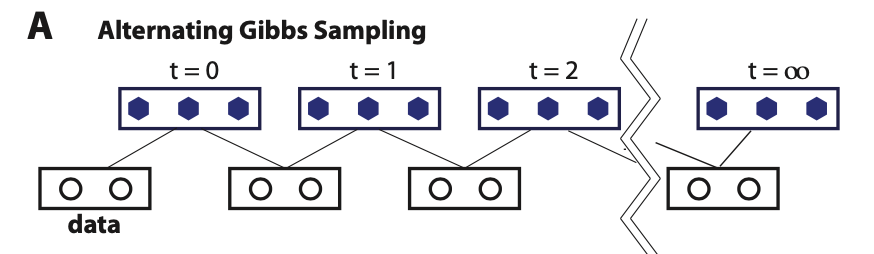
\includegraphics[width = 0.5\textwidth]{Slides/Trainning3.png}\hspace{3cm}figure from \cite{Mehta2019}
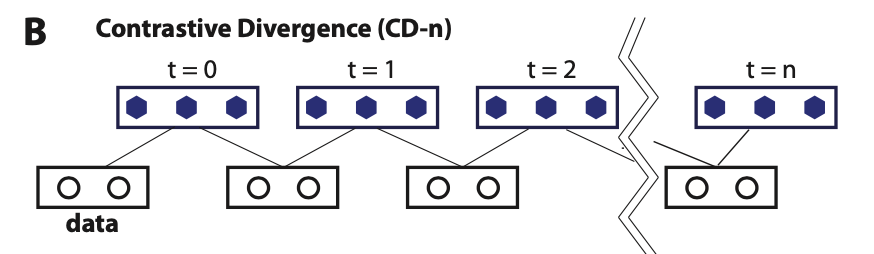
\includegraphics[width = 0.5\textwidth]{Slides/Training2.png}
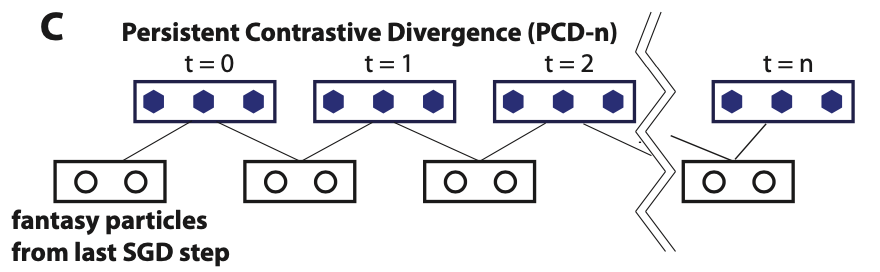
\includegraphics[width = 0.45\textwidth]{Slides/Trainning1.png}

\end{frame}



\section{At/Out of equilibrium Boltzmann machines}
\begin{frame}{At/Out of equilibrium Boltzmann machines}
Algorithm for equilibrium sampling: 
\begin{itemize}
    \item[1.] Start from an initial point and make many Gibbs steps until equilibrium
    \item[2.] Repeat for each particle in the batch
    \item[3.] Compute the gradients on the batch
    \item Most of the time this procedure is too slow. And we are not sampling the equilibrium distribution.
    \item Most of the time 1-5 steps of Gibbs sampling are sufficient for each predictions
\end{itemize}

\end{frame}


\subsection{Training an RBM in and out of equilibrium}
\begin{frame}{Training an RBM in and out of equilibrium}{Training at equilibrium}
Set up: \hspace{5cm} 
\begin{itemize}
    \item[•] "And" data $\rightarrow$ 111, 100, 010, 000
    \item[•] Visible layer $N_v = 3$
    \item[•] hidden layer $N_h = 3$
    \item[•] Discrete hidden and visible variables in $\{0, 1\}$
\end{itemize}

\vspace*{-0.5em}
\begin{figure}
\centering
\begin{minipage}{.5\textwidth}
  \centering
  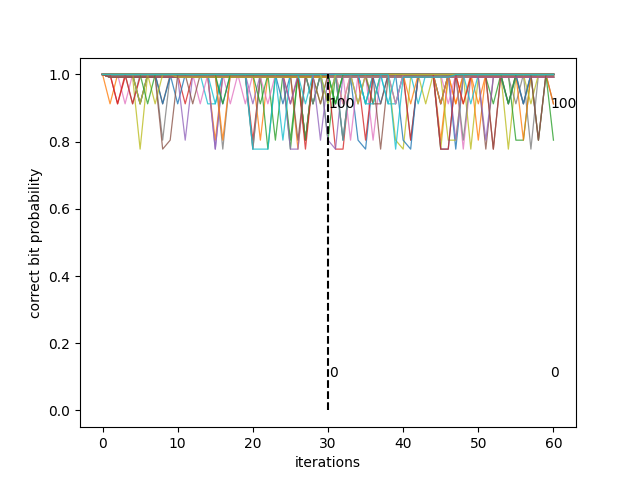
\includegraphics[width=.99\linewidth]{Slides/rbm_bit_stability_short.png}
  \caption{\vspace*{-1em}valid state retention}
  \label{fig:test1}
\end{minipage}%
\begin{minipage}{.5\textwidth}
  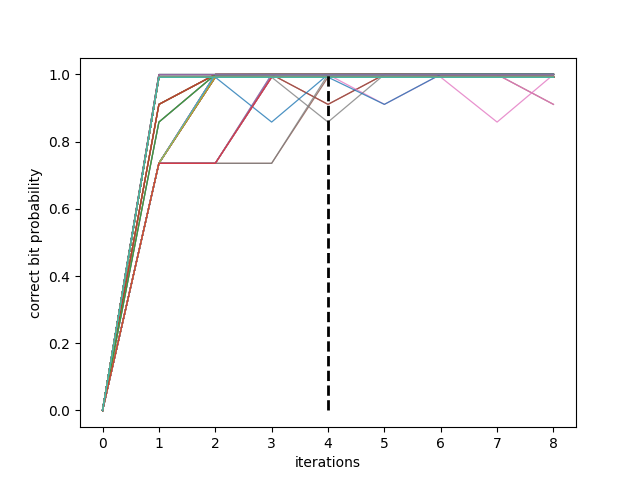
\includegraphics[width=.99\linewidth]{Slides/rbm_bit_correction_short.png}
  \caption{\vspace*{-1em}error state correction}
  \label{fig:test2}
\end{minipage}
\end{figure}
\end{frame}

\subsection{Out of equilibrium}

\subsection{Training and sampling an out of equilibrium RBM}

\begin{frame}{At and out of equilibrium}{Trainning and sampling an out of equilibrium RBM - MNIST}
Pseudo-continuous RBM from discrete RBM:
\begin{itemize}
    \item $N_v = 28\times28$ discrete visible variables
    \item discrete hidden layer with $N_h = 500$
    \item using bit probability as continuous output 
    \item using random sampling as continuous input for training
\end{itemize}
    
\begin{figure}
\centering
\begin{minipage}{.5\textwidth}
  \centering
  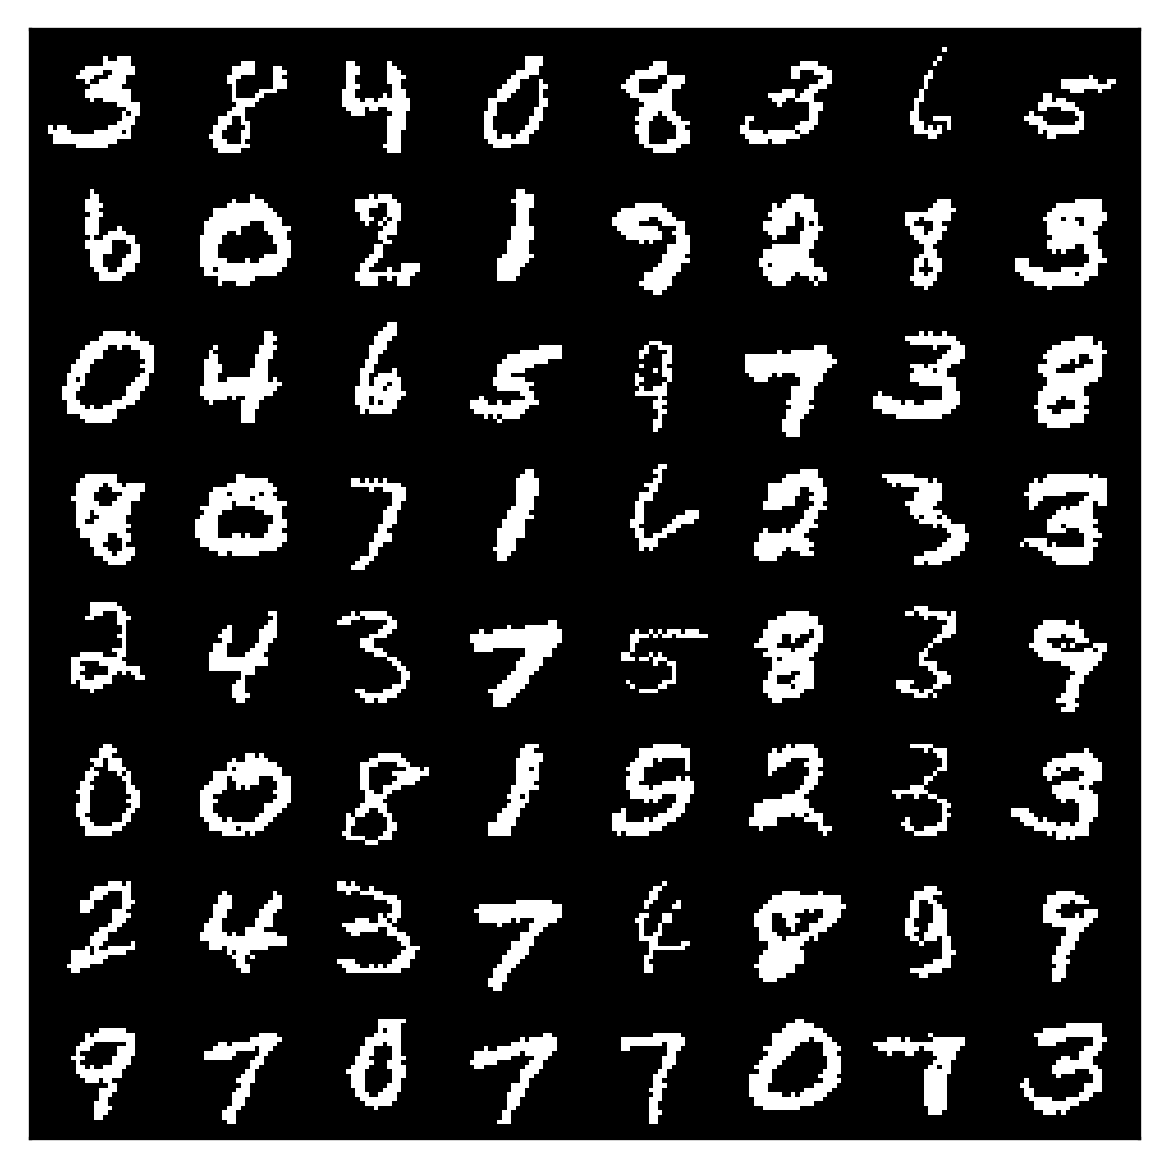
\includegraphics[width=.99\linewidth]{Slides/real_mnist.png}
  \caption{Real data\vspace*{1em}}
  \label{fig:test1}
\end{minipage}%
\begin{minipage}{.5\textwidth}
  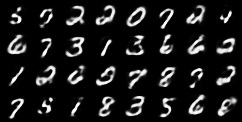
\includegraphics[width=.99\linewidth]{Slides/generate_mnist.png}
  \caption{Generated data (pixel probabilities)}
  \label{fig:test2}
\end{minipage}
\end{figure}

\end{frame}


\begin{frame}{At and out of equilibrium}{Trainning and sampling an out of equilibrium RBM - MNIST}

\vspace*{-0.5em}

\begin{itemize}
    \item[•] Initialise with random noise
    \item[•] The Machine tends to generate something that "looks like" the data
\end{itemize}
\begin{figure}
  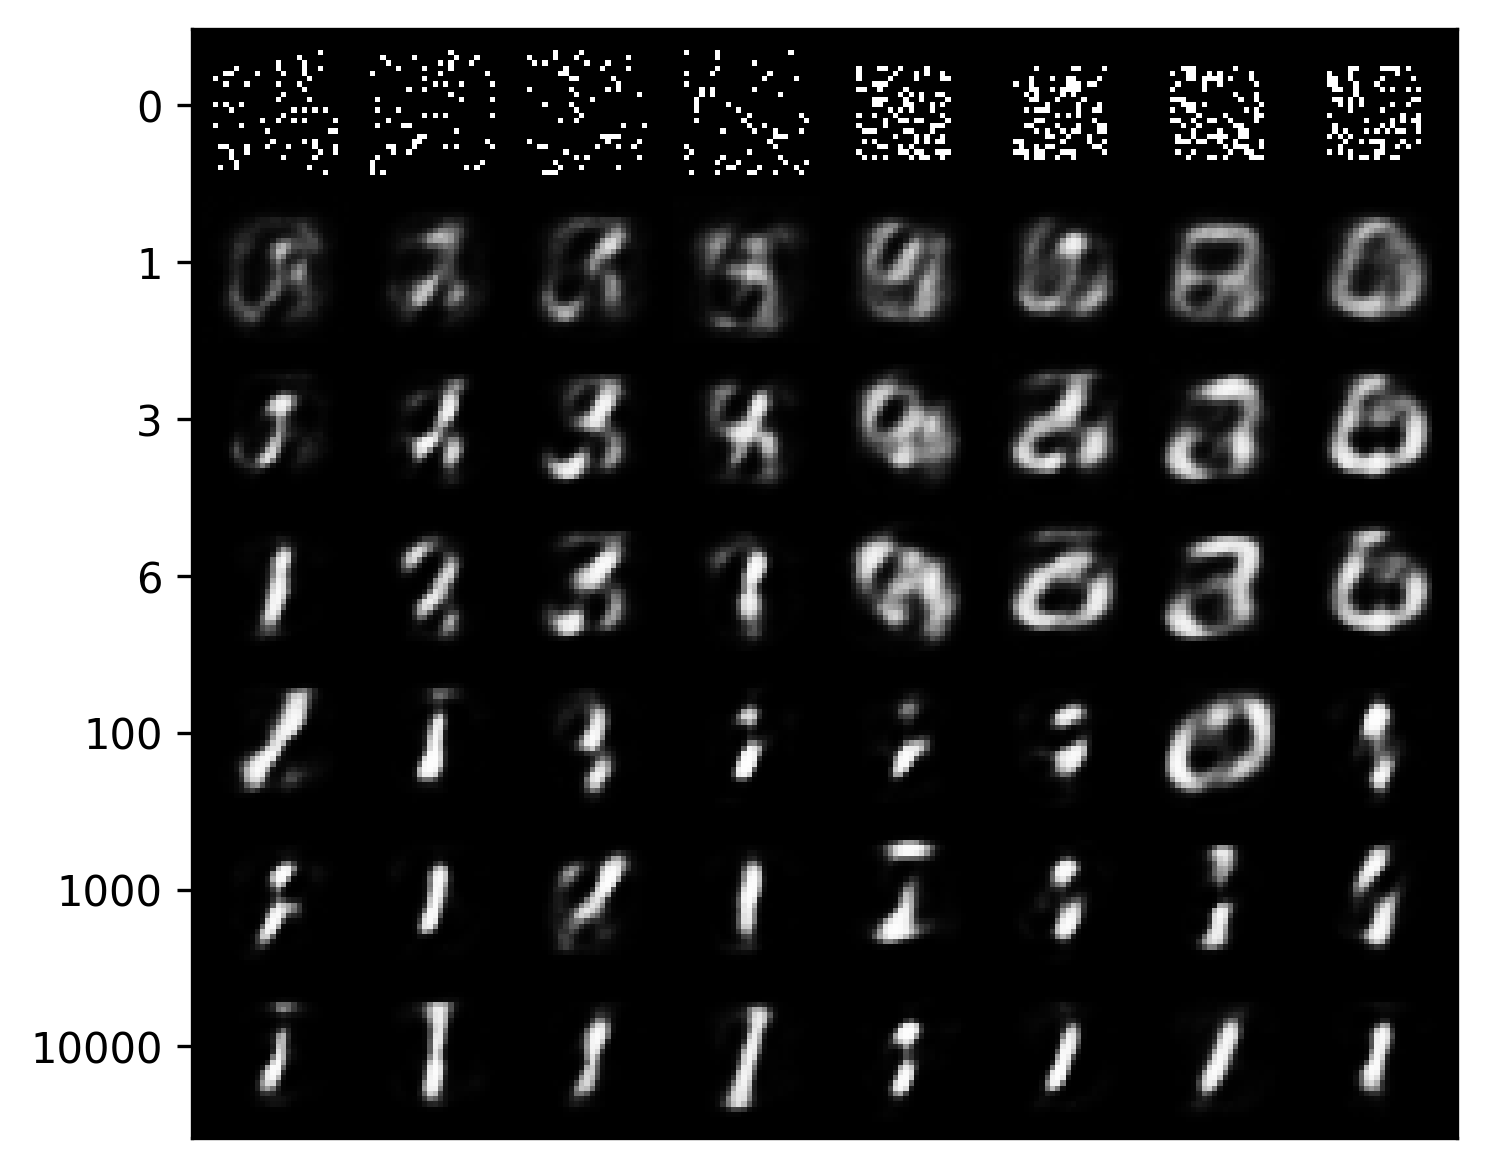
\includegraphics[width=.6\linewidth]{Slides/generate_mnist_steps.png}
  \caption{Generated data (pixel probabilities) - starting from random noise and over iterations}
  \label{fig:test2}
\end{figure}

\end{frame}


\begin{frame}{At and out of equilibrium}{Trainning and sampling an out of equilibrium RBM - MNIST Fashion}

$\Delta_E = E(v_0) - E(v_n) \rightarrow 0$ because $v_0$ is becoming a local optimum, thus $v_0$ is a stable point and $\Delta_E = 0$

\begin{figure}
  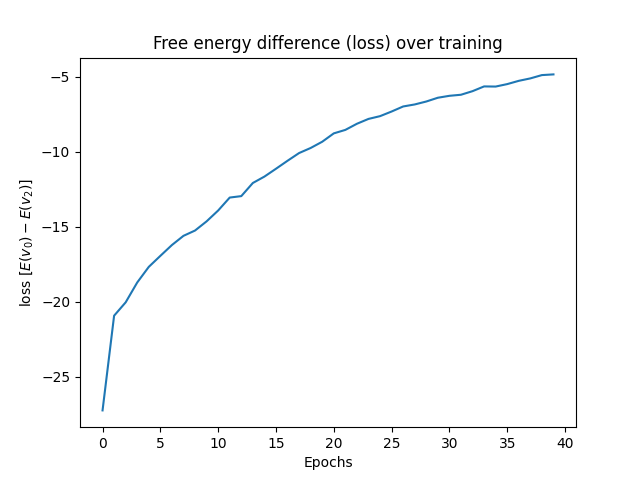
\includegraphics[width=.8\linewidth]{Slides/free_energy_fashion.png}
  \label{fig:test2}
\end{figure}

\end{frame}




\begin{frame}{At and out of equilibrium}{Trainning and sampling an out of equilibrium RBM - MNIST Fashion}

Real vs generated data (same setup as for MNIST):
    
\begin{figure}
\centering
\begin{minipage}{.5\textwidth}
  \centering
  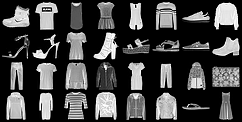
\includegraphics[width=.99\linewidth]{Slides/real_fashion.png}
  \caption{Real data\vspace*{1em}}
  \label{fig:test1}
\end{minipage}%
\begin{minipage}{.5\textwidth}
  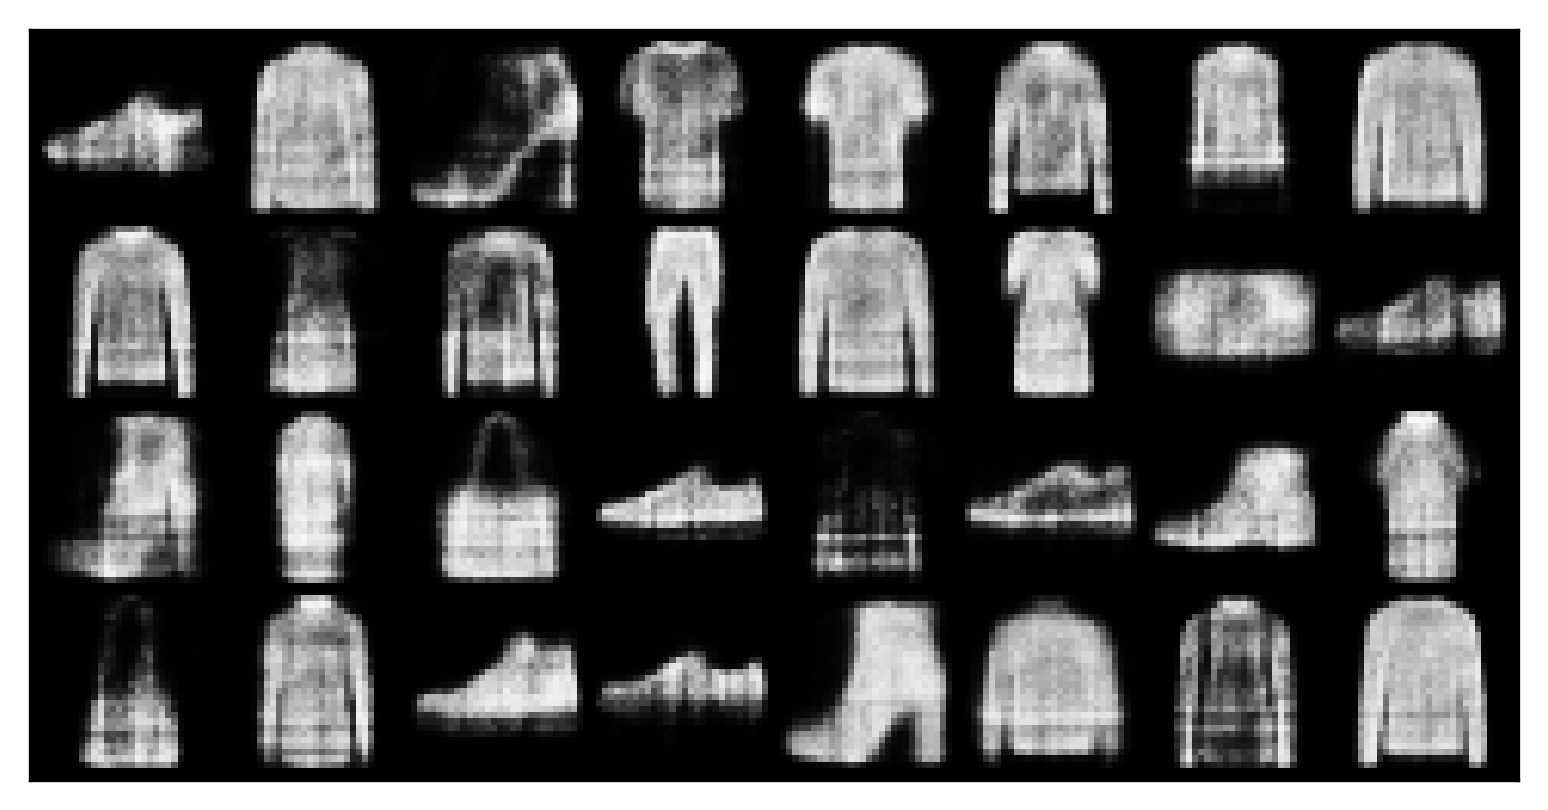
\includegraphics[width=.99\linewidth]{Slides/generate_fashion.png}
  \caption{Generated data (pixel probabilities)}
  \label{fig:test2}
\end{minipage}
\end{figure}

\end{frame}


\begin{frame}{At and out of equilibrium}{Trainning and sampling an out of equilibrium RBM - MNIST Fashion}
The Boltzmann Machine (as Hopfield) network is able to memorise and retrive patterns.
The image that were used for the training becomes attractors for the dynamics of the Boltzmann machine.

\begin{figure}
  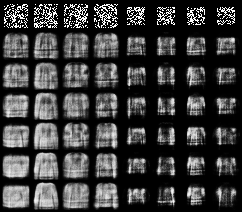
\includegraphics[width=.6\linewidth]{Slides/generate_fashion_steps.png}
  \caption{Generated data (pixel probabilities) - starting from random noise and over iterations}
  \label{fig:test2}
\end{figure}

\end{frame}

\section{RBM as a Langevin Process}
\subsection{Learning a Langevin Process}
\begin{frame}{RBM as a langevin process}{Mearning as a langevin process}
There is some litterature on that : \cite{Agoritsas2023}, \cite{Decelle2018}, \cite{Decelle2022}.

\begin{theorem}
    Let be $f_\theta$ an observable conjugated with the parameter $\theta$ and let us suppose that there exist a set of parameter such that $\nabla \mathcal{L}=0$ then if we generate sample with the exact same procedure as the training, it represent correctly the statistics of the data.
\end{theorem}

\begin{theorem}
    In the same way if $\nabla \mathcal{L}=\epsilon$, if we sample the model in the same procedure as the training, we will have an error of order $\epsilon$ on the observable. For a sufficiently small $\epsilon$ it is possible to find $k^{\dagger}$ such that the error on $\left< f_{\theta^{\dagger},i}\right> vanishes.$
\end{theorem}
    
\end{frame}

\section*{Conclusion}

\begin{frame}{Bibliography}[allowframebreaks]
    \bibliography{Slides/bibliography.bib}
    \bibliographystyle{unsrt}
\end{frame}

\end{document}